% Overleaf: upload this file and the figures/ directory; use pdfLaTeX.
% Includes the cover, contents and references; compile twice for page references.
\documentclass[a4paper,10pt]{article}
\usepackage[top=17mm,bottom=18mm,left=18mm,right=18mm,headheight=14pt,headsep=6mm,footskip=10mm]{geometry}
\usepackage[T1]{fontenc}
\usepackage[utf8]{inputenc}
\usepackage{mathpazo}
\usepackage[scaled=.94]{helvet}
\usepackage{microtype,graphicx,xcolor,amsmath,amssymb,booktabs,tabularx,array,multicol}
\usepackage{caption,fancyhdr,enumitem,titlesec,tcolorbox,listings,hyperref}
\definecolor{teal}{HTML}{176B70}
\definecolor{gold}{HTML}{AD762A}
\definecolor{ink}{HTML}{203440}
\definecolor{muted}{HTML}{5B6F79}
\definecolor{pale}{HTML}{EAF2F2}
\definecolor{warm}{HTML}{F6F0E6}
\hypersetup{colorlinks=true,linkcolor=teal,urlcolor=teal,citecolor=teal,
 pdftitle={Interactive Automotive Chain Reaction},pdfauthor={Mohammad Moin Uddin Moin},
 pdfsubject={CSE 4102: Computer Graphics and Image Processing Laboratory}}
\setlength{\parindent}{0pt}
\setlength{\emergencystretch}{2em}
\setlength{\parskip}{5pt}
\setlength{\tabcolsep}{5pt}
\renewcommand{\arraystretch}{1.1}
\AtBeginEnvironment{tabularx}{\fontsize{9.3}{11.5}\selectfont}
\AtBeginEnvironment{tabular}{\fontsize{9.3}{11.5}\selectfont}
\setlist[itemize]{leftmargin=14pt,itemsep=2pt,topsep=3pt}
\setlist[enumerate]{leftmargin=17pt,itemsep=2pt,topsep=3pt}
\captionsetup{hypcap=false,font={small},labelfont={bf,color=teal},justification=raggedright,singlelinecheck=false,skip=3pt}
\titleformat{\section}{\sffamily\Large\bfseries\color{ink}}{\textcolor{teal}{\thesection}}{.6em}{}
\titlespacing*{\section}{0pt}{0pt}{7pt}
\titleformat{\subsection}{\sffamily\normalsize\bfseries\color{teal}}{}{0pt}{}
\titlespacing*{\subsection}{0pt}{8pt}{3pt}
\pagestyle{fancy}\fancyhf{}
\fancyhead[L]{\sffamily\footnotesize\color{muted}INTERACTIVE AUTOMOTIVE CHAIN REACTION}
\fancyhead[R]{\sffamily\footnotesize\color{muted}CSE 4102}
\fancyfoot[R]{\sffamily\footnotesize\color{teal}\thepage\ / \pageref*{report:lastpage}}
\renewcommand{\headrulewidth}{.3pt}
\renewcommand{\footrulewidth}{0pt}
\newcommand{\StudentName}{Mohammad Moin Uddin Moin}
\newcommand{\StudentRoll}{2107111}
\newcommand{\SubmissionDate}{11 October 2026}
\newcommand{\code}[1]{\texttt{\detokenize{#1}}}
\newcommand{\lead}[1]{{\sffamily\color{muted}\normalsize #1\par}\vspace{3pt}}
\newcommand{\reportpage}[2]{\newpage\section{#1}\label{section:\thesection}\lead{#2}}
\newcommand{\pic}[3]{\begin{center}\includegraphics[width=\linewidth,height=#2,keepaspectratio]{figures/#1}\captionof{figure}{#3}\end{center}}
\newcommand{\twoshots}[5]{\par\noindent\begin{minipage}[t]{.487\linewidth}\vspace{0pt}\pic{#1}{#5}{#2}\end{minipage}\hfill\begin{minipage}[t]{.487\linewidth}\vspace{0pt}\pic{#3}{#5}{#4}\end{minipage}\par}
\newcommand{\threepics}[6]{\par\noindent\begin{minipage}[t]{.32\linewidth}\vspace{0pt}\pic{#1}{42mm}{#2}\end{minipage}\hfill\begin{minipage}[t]{.32\linewidth}\vspace{0pt}\pic{#3}{42mm}{#4}\end{minipage}\hfill\begin{minipage}[t]{.32\linewidth}\vspace{0pt}\pic{#5}{42mm}{#6}\end{minipage}\par}
\newtcolorbox{keyidea}{colback=pale,colframe=teal,boxrule=.4pt,arc=1mm,left=7pt,right=7pt,top=5pt,bottom=5pt,before skip=6pt,after skip=6pt}
\newtcolorbox{notebox}{colback=warm,colframe=gold,boxrule=.35pt,arc=1mm,left=7pt,right=7pt,top=5pt,bottom=5pt,before skip=6pt,after skip=6pt}
\newcolumntype{Y}{>{\raggedright\arraybackslash}X}
\newcommand{\tagline}[1]{{\sffamily\small\bfseries\color{teal}#1\par}}
\lstset{basicstyle=\ttfamily\footnotesize,breaklines=true,columns=fullflexible,keepspaces=true,
 backgroundcolor=\color{pale},frame=single,rulecolor=\color{pale},xleftmargin=4pt,xrightmargin=4pt,
 aboveskip=5pt,belowskip=5pt,showstringspaces=false}
\numberwithin{equation}{section}
\begin{document}
\fontsize{10.5}{13.4}\selectfont
% ------------------------------- 01 / COVER
\thispagestyle{empty}
\begin{center}
{\sffamily\large\bfseries Khulna University of Engineering \& Technology}\\[4pt]
{\sffamily Department of Computer Science and Engineering}\\[13pt]
{\sffamily\color{teal}\bfseries CSE 4102}\\[3pt]
{\sffamily Computer Graphics and Image Processing Laboratory}\\[12pt]
{\sffamily\small FINAL PROJECT REPORT}\\[13pt]
{\sffamily\fontsize{28}{32}\selectfont\bfseries\color{ink}Interactive Automotive\\Chain Reaction}\\[7pt]
{\sffamily\color{muted}A primitive-built 3D machine with seventeen connected actions,\\interactive controls, and a drivable car}
\end{center}
\vspace{2mm}
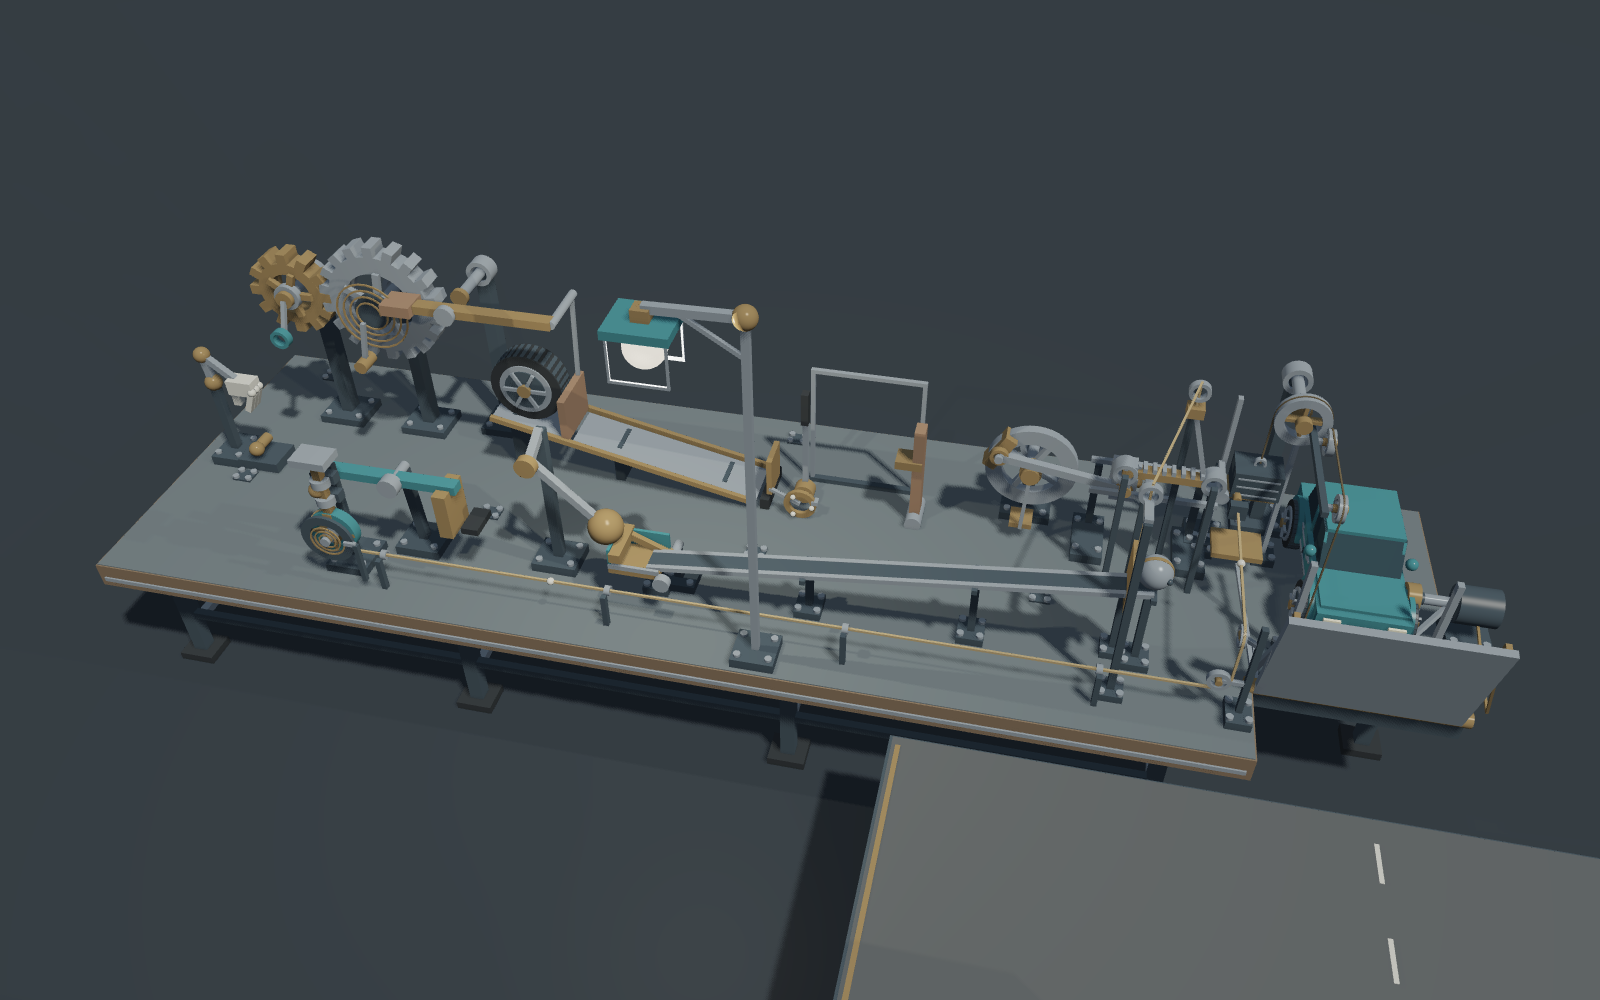
\includegraphics[width=\linewidth]{figures/overview.png}
\vspace{3mm}
\begin{center}{\sffamily\small\color{teal}\bfseries
TRIANGLES, CUBES \& SPHERES \quad | \quad 70-SECOND RELEASE \quad | \quad OPENGL 3.3}
\end{center}
\vspace{4mm}
\par\noindent\begin{minipage}[t]{.49\linewidth}\vspace{0pt}
\tagline{SUBMITTED BY}
\textbf{\StudentName}\\
Roll: \StudentRoll\\
Department of CSE, KUET
\end{minipage}\hfill
\begin{minipage}[t]{.47\linewidth}\vspace{0pt}
\tagline{SUBMITTED TO}
\textbf{Md Tajmilur Rahman}\\Lecturer, Department of CSE, KUET\par
\textbf{Md. Mubtashim Abrar Nihal}\\Lecturer, Department of CSE, KUET
\end{minipage}\par
\vfill
\begin{center}{\sffamily\color{muted}\SubmissionDate}\end{center}

% ------------------------------- 02 / ABSTRACT
\newpage
\section*{Abstract and project at a glance}
\lead{One machine makes the graphics concepts visible: build the parts, animate their contacts, illuminate them, and let the user take control.}
This project is an interactive three-dimensional automotive workshop machine implemented in C++17 and OpenGL 3.3. A glove inserts a starter pin, a gear train winds a spring, and a sequence of rolling, rotating and sliding mechanisms eventually clears a car's exit. Seventeen scheduled actions reach the car-release condition at \textbf{70 active seconds}; presentation mode then drives the car onto the apron over seven more seconds.

Every object is assembled procedurally from cubes, spheres and explicitly generated triangle meshes. Model, view and projection matrices place the geometry on screen. A visible inspection lamp supplies a point light; two presets additionally use directional sunlight. The renderer supports Gouraud, Phong and face-normal shading, source-specific shadow maps, and an optional CPU ray-traced still image.
\pic{overview_ui}{91mm}{The actual application at the beginning of the chain. The top bar selects mode and opens the guide. The bottom bar reports the current action, active time, lock state and available controls.}
\par\noindent\begin{tabularx}{\linewidth}{@{}Y Y Y@{}}
\toprule
\textbf{Observe} & \textbf{Operate} & \textbf{Inspect}\\
Automatic 17-action presentation; visible contacts and a final car exit. & Hold/tap controls for five mechanisms; ordered releases for the remaining actions; arrow-key driving. & Six camera presets and free movement; lighting/shading comparison; ray-traced snapshot.\\
\bottomrule
\end{tabularx}\par
\begin{keyidea}
\textbf{The causal story:} insertion and winding $\rightarrow$ wheel and wiper $\rightarrow$ crank and ball $\rightarrow$ cup, striker and pin $\rightarrow$ cable and counterweight $\rightarrow$ bridge and starter $\rightarrow$ car departure.
\end{keyidea}
The mechanism uses authored kinematics with contact and clearance guards. This makes it deterministic and explainable: the report distinguishes geometric constraints, interaction logic and illumination calculations from a full force-based simulation.

% ------------------------------- 03 / CONTENTS
\newpage
\section*{Contents and assessment map}
\lead{Read pages 2, 4, 9 and 10--12 first to understand the complete machine. The remaining pages explain how that result is computed.}
\par\noindent\begin{tabularx}{\linewidth}{@{}p{10mm}Y r@{}}
\toprule
 & \textbf{Topic} & \textbf{Page}\\\midrule
 & Abstract and project at a glance & 2\\
1 & Scene layout and the visible chain & \pageref{section:1}\\
2 & Primitive geometry: from vertices to reusable meshes & \pageref{section:2}\\
3 & Building the automotive mechanisms & \pageref{section:3}\\
4 & Constructing the front relay & \pageref{section:4}\\
5 & Car, glove, workbench and inspection lamp & \pageref{section:5}\\
6 & Complete stage schedule & \pageref{section:6}\\
7 & How the first seven actions connect & \pageref{section:7}\\
8 & Ball-to-drum relay: contacts and clearances & \pageref{section:8}\\
9 & Final release: catch, barrier, bridge and starter & \pageref{section:9}\\
10 & 3D transformation mathematics & \pageref{section:10}\\
11 & Hierarchies, pivots and normal transformation & \pageref{section:11}\\
12 & Motion functions and geometric constraints & \pageref{section:12}\\
13 & Logic, time and reset behavior & \pageref{section:13}\\
14 & 3D viewing and the free camera & \pageref{section:14}\\
15 & Perspective projection, clipping and screen mapping & \pageref{section:15}\\
16 & Lighting design and selectable environments & \pageref{section:16}\\
17 & Illumination: the implemented Phong equation & \pageref{section:17}\\
18 & Materials and the complete RGB calculation & \pageref{section:18}\\
19 & Shadow mapping and visibility & \pageref{section:19}\\
20 & Gouraud, Phong and face-normal shading & \pageref{section:20}\\
21 & CPU ray tracing: a second rendering path & \pageref{section:21}\\
22 & Interactive operation and the demo guide & \pageref{section:22}\\
23 & Keyboard car driving and the controls chart & \pageref{section:23}\\
24 & Program architecture and the rendering pipeline & \pageref{section:24}\\
25 & Verification and measured evidence & \pageref{section:25}\\
26 & Demonstration plan, results and limitations & \pageref{section:26}\\
27 & Conclusion and references & \pageref{section:27}\\
\bottomrule
\end{tabularx}\par
\vspace{3mm}
\textbf{Notation.} Bold symbols denote vectors; $T,R,S$ denote translation, rotation and scale matrices; $M,V,P$ denote model, view and projection matrices. $t$ is active simulation time, $u$ is normalized stage progress, and $\Delta t$ is elapsed time. Distances are in \emph{scene units}; no conversion to metres or physical energy units is claimed.

% ------------------------------- 04 / LAYOUT
\reportpage{Scene layout and the visible chain}{The sequence crosses the back row, returns along the front row, then carries its release signal to the car bay.}
\pic{scene_map}{91mm}{Plan view using the project's world $x$--$z$ coordinates. The numbered markers identify actions; arrows explain their order. Marker 13 is displaced left for readability; its drum axis is at $x=-7.815$. The apron continues beyond the cropped plan.}
\par\noindent\begin{tabularx}{\linewidth}{@{}p{27mm}Y Y@{}}
\toprule
\textbf{Region} & \textbf{What the reader sees} & \textbf{Role in the chain}\\\midrule
Back row, 1--7 & Glove, meshing gears, cam/lever, ramp wheel, wiper, clutch bar, crank/slider. & Initiates motion and raises the stop that holds the relay ball.\\
Front row, 8--13 & Sloped ball track, captive cup, striker, rocker, sliding pin and spring drum. & Converts rolling motion into successive hinge, slider and cable actions.\\
Right side, 14--17 & Catch, guided weight, overhead cable, barrier, drawbridge and starter. & Clears the car roof and roadway, then withdraws the starter and tire shoe.\\
Car and apron & Car bay, hinge bridge, marked driving area. & The visible output; arrows can drive the released car.\\
\bottomrule
\end{tabularx}\par
\subsection*{Coordinate system and useful landmarks}
The world is right-handed. $+y$ points upward; $+z$ points toward the front relay and the car's exit. Most front-facing mechanisms rotate in the $xy$ plane about a local $z$ axis. The bridge rotates about $x$; car steering and chassis heading rotate about $y$.
\begin{keyidea}
\textbf{Three landmarks:} the crank centre is $(3.55,1.55,0.10)$; the cup pivot is $(-2.10,0.80,3.15)$; the visible lamp and point-light centre both equal $(-1.80,5.80,4.10)$.
\end{keyidea}
The stepped workbench supports the entire machine while leaving a real gap under the drawbridge. The large floor and the apron establish depth and a destination for the car. Camera presets 1, 5 and 6 reveal the overall path, front relay and small contacts respectively.

% ------------------------------- 05 / PRIMITIVES
\reportpage{Primitive geometry: from vertices to reusable meshes}{A complicated object is a collection of small transformed meshes. Every rendered surface ultimately reaches OpenGL as triangles.}
\pic{primitives}{53mm}{Construction diagrams reproducing the reusable mesh topology. A cylinder or ring is explicitly assembled from triangles; it is not an imported solid or external model. Wire edges explain construction and are not a normal application display mode.}
\par\noindent\begin{tabularx}{\linewidth}{@{}p{30mm}p{24mm}Y@{}}
\toprule
\textbf{Reusable mesh} & \textbf{Triangles} & \textbf{Generation rule and use}\\\midrule
Unit cube & $6\times2=12$ & Corners in $[-\tfrac12,\tfrac12]^3$; two triangles per face. Beams, teeth, panels and supports.\\
Sphere & $2(16-1)24=720$ & 16 latitude intervals, 24 longitude intervals; omit degenerate pole triangles. Balls and joints.\\
Disk/cylinder & $48\times4=192$ & 48 circular segments; two side triangles and two cap triangles per segment. Axles, hubs and tires.\\
Full annulus & $64\times8=512$ & Outer/inner walls and two annular caps; inner radius $0.65$ of outer radius. Rims and pulleys.\\
Half annulus & $512+4=516$ & Same 64 segments over $\pi$ radians, with four closing triangles. Car wheel arches.\\
Cabin wedge & $12$ & Eight custom corners; six triangulated faces make sloped glazing.\\
Subdivided cube & $12d^2$ & $d=16$ or $64$ gives 3,072 or 49,152 triangles; improves Gouraud sampling on large surfaces.\\
\bottomrule
\end{tabularx}\par
\subsection*{Position and normal construction}
For a unit sphere, sampled angles $\phi=\pi j/16$ and $\theta=2\pi i/24$ give
\begin{equation}
\mathbf p(\phi,\theta)=(\sin\phi\cos\theta,\cos\phi,\sin\phi\sin\theta),\qquad \mathbf n=\mathbf p.
\end{equation}
A cylinder uses $(\cos\theta,\sin\theta,\pm0.5)$, with radial side normals $(\cos\theta,\sin\theta,0)$ and separate cap normals. For a planar triangle,
\begin{equation}
\mathbf n_f=\frac{(\mathbf b-\mathbf a)\times(\mathbf c-\mathbf a)}{\|(\mathbf b-\mathbf a)\times(\mathbf c-\mathbf a)\|}.
\end{equation}
The vertex record contains a position and normal. Vertices are uploaded once to VBOs, described by VAOs, and drawn with \code{GL_TRIANGLES}. Repeated objects reuse the mesh while supplying their own model matrix and material.

% ------------------------------- 06 / ASSEMBLY
\reportpage{Building the automotive mechanisms}{Repeat simple geometry around an axle, then attach the whole assembly to one transform.}
\pic{gear_assembly}{57mm}{Front-view construction of a small gear: triangle-built ring, repeated cube teeth, cube spokes, hub and support. This explanatory drawing separates the roles of the primitives.}
\twoshots{gear}{Actual gear train and exposed spring at $t=8$ s.}{crank}{Actual crank, fixed-length rod, slider and rack at $t=26.5$ s.}{54mm}
\par\noindent\begin{tabularx}{\linewidth}{@{}p{29mm}Y Y@{}}
\toprule
\textbf{Object} & \textbf{Construction} & \textbf{Placement / motion}\\\midrule
Gear pair & 12/18 cube teeth, five cube spokes per gear, annular rims and disk hubs. & Radii $0.70/1.05$; centres $x=-10,-8.25$ at $y=3.25$. Angles obey $\theta_s=-1.5\theta_l$.\\
Rolling wheel & Triangle tire, hub disks, six cube spokes on each side and 32 cube tread marks. & Radius $0.68$; translation follows the ramp and tread rotation makes rolling readable.\\
Cam and lever & Disk centre, offset roller, cube-based connecting beam and long lever. & Cam rotates $150^\circ$; the lever turns $-32^\circ$ and retracts the stop.\\
Wiper and bar & Narrow arm/blade cubes, disk pivot, cube windshield frame and clutch bar. & One $-65^\circ$ wiper sweep; one $-84^\circ$ bar rotation presses the pedal.\\
Crank/slider & Annular crank, four spokes, offset pin, oriented cube rod and piston block. & Rotation becomes linear motion while preserving the $2.15$-unit rod length.\\
\bottomrule
\end{tabularx}\par
\subsection*{One rule creates every repeated tooth}
For tooth $i$, the local rotation is $\alpha_i=2\pi i/N$. Its model matrix is
\begin{equation}
M_i=T(\mathbf c)R_z(\theta)R_z(\alpha_i)T(r,0,0)S(0.19,0.18,0.40).
\end{equation}
The first two factors move the complete gear. The next factors arrange the teeth around it. Spring curves and thin cables are sequences of short, oriented cube beams; they show transmission and stored-energy intent without adding a spring-force solver.

% ------------------------------- 07 / RELAY CONSTRUCTION
\reportpage{Constructing the front relay}{Six visibly different components use a small set of meshes and six clear mechanical roles.}
\pic{relay_1}{76mm}{The front relay during cup tipping at $t=37.1$ s. Read right to left: loaded cup, pendulum striker, rocker, pin and drum. The ball track enters from the right; the low cable returns toward the far-right catch.}
\par\noindent\begin{tabularx}{\linewidth}{@{}p{24mm}Y Y@{}}
\toprule
\textbf{Component} & \textbf{Primitive construction} & \textbf{Motion and purpose}\\\midrule
Rolling ball & Radius-$0.27$ sphere, thin annular brass stripe and small spherical marker. & Translates 8.22 scene units down the track; the stripe rotates by distance/radius.\\
Trigger cup & Cube floor $(0.86,0.10,0.72)$, side cheeks, retaining finger and disk axle. & Turns $32^\circ$ about its right pivot, carrying the captured ball and removing the striker stop.\\
Pendulum & Cube rod of length $1.65$, radius-$0.30$ spherical bob and disk pivot. & Swings once from $+45^\circ$ to $-45^\circ$ to meet the rocker pad.\\
Rocker arm & Cube beam $(2.30,0.16,0.24)$, pad, shaft and spherical roller. & Turns $-25^\circ$; the roller reaches the collar of the sliding pin.\\
Sliding pin & Cube shaft $(0.14,1.30,0.15)$, cube collar and two guides. & Rises $0.65$ units, clearing the spring drum's rim.\\
Cable drum & Radius-$0.42$ ring, four spokes, spiral beam spring and wrapped beam cable. & Takes up $0.70$ units of cable and withdraws the remote catch bolt.\\
\bottomrule
\end{tabularx}\par
\subsection*{A captive ball and a fixed-length striker}
Once the ball is seated, its local coordinate is retained in the cup:
\begin{equation}
\mathbf b(t)=T(\mathbf c)R_z(\theta_c(t))(\mathbf b_{\rm seated}-\mathbf c).
\end{equation}
The striker centre is $T(\mathbf p)R_z(\theta_p)(0,-1.65,0)^T$. The rod and spherical bob share this transform, so the arm cannot stretch. Similarly, the rocker pad and roller belong to a single rocker transform.
\begin{keyidea}
Each part changes the kind or location of motion: rolling $\rightarrow$ tipping $\rightarrow$ swinging $\rightarrow$ rocking $\rightarrow$ sliding $\rightarrow$ cable take-up.
\end{keyidea}

% ------------------------------- 08 / VEHICLE AND CONTEXT
\reportpage{Car, glove, workbench and inspection lamp}{The final vehicle and the starting glove use the same primitive and hierarchy rules as the machine.}
\twoshots{car_model}{Isolated car rendered with the application's original \code{Scene::car()} geometry.}{glove_place}{Glove after carrying the pin to its socket, $t=4.5$ s.}{58mm}
\par\noindent\begin{tabularx}{\linewidth}{@{}p{25mm}Y Y@{}}
\toprule
\textbf{Assembly} & \textbf{How it is built} & \textbf{Purpose / behavior}\\\midrule
Car body & Cube chassis, floor, hood, roof, bumpers, grille, trim and light housings; triangulated sloped cabin; sphere mirrors. & All inherit the chassis translation and yaw. The dark cabin material suggests glazing but is opaque.\\
Car wheels & Four radius-$0.43$ triangle tires, spoke cubes, disk hubs, tread cubes and half-annulus fenders. & Front wheels steer; all wheels roll using signed travel. Reverse travel reverses their spin.\\
Starter socket & Ring and disk hub mounted on the car, with a visible orientation bar. & Aligns with the external shaft; cranks before release and remains with the car afterward.\\
Glove and arm & Cube palm, three finger cubes, thumb cube, sphere knuckles, two arm beams and sphere joints. & Picks up one designated pin, carries it at a fixed hand offset, places it, then withdraws.\\
Workbench & Scaled cube slabs, edge strips, legs, feet, cross-braces and bolted mounts. & Supports the chain and exposes the bridge gap. Small material differences separate frame, top and contacts.\\
Inspection lamp & Cube clamp and shade, beam supports, spherical joint and radius-$0.32$ emissive bulb. & The visible bulb centre is the actual point light. Clicking its bulb or guard changes the preset.\\
\bottomrule
\end{tabularx}\par
\subsection*{Glove pickup has an explicit attachment interval}
During the middle half of the six-second glove stage, the pin is attached:
\begin{equation}
\mathbf p_{\rm pin}=\mathbf p_{\rm hand}+(0,-0.40,0),\qquad 0.25\le u_{\rm glove}<0.75.
\end{equation}
Before pickup it rests on the tray; after placement it stays at $(-10,2.68,0.82)$. The three fingers rotate as the grip closes. The arm follows an authored pose; arbitrary object grabbing and inverse kinematics are outside this implementation.
\begin{notebox}
\textbf{Modeling scope:} material color, mesh shape and specular response provide the appearance. No imported mesh models, image surface textures, transparent cabin rendering or headlight light sources are claimed.
\end{notebox}

% ------------------------------- 09 / TIMING
\reportpage{Complete stage schedule}{Seventeen meaningful actions occupy seventy active seconds. The automatic car exit is an additional seven seconds.}
\par\noindent\begin{minipage}[t]{.50\linewidth}\vspace{0pt}
\small
\par\noindent\begin{tabular}{@{}r l r r@{}}
\toprule
\textbf{No.}&\textbf{Action}&\textbf{Interval}&\textbf{Duration}\\\midrule
1&Glove&0--6&6 s\\
2&Gears&6--10&4 s\\
3&Cam / lever&10--14&4 s\\
4&Rolling wheel&14--18&4 s\\
5&Wiper&18--21&3 s\\
6&Clutch bar&21--24&3 s\\
7&Crank / ball stop&24--29&5 s\\
8&Rolling ball&29--36&7 s\\
9&Trigger cup&36--39&3 s\\
10&Pendulum&39--43&4 s\\
11&Rocker arm&43--45&2 s\\
12&Sliding pin&45--47&2 s\\
13&Cable drum / bolt&47--50&3 s\\
14&Catch&50--53&3 s\\
15&Counterweight&53--58&5 s\\
16&Drawbridge&58--65&7 s\\
17&Starter / shoe&65--70&5 s\\\midrule
&\textbf{Car released}&\textbf{70}&\\
&Automatic exit&70--77&7 s\\
\bottomrule
\end{tabular}\par
\end{minipage}\hfill
\begin{minipage}[t]{.46\linewidth}\vspace{0pt}
\subsection*{What counts as time?}
Active time advances while the simulation is running. Pausing, waiting for interactive input, and computing a ray-traced snapshot add wall-clock time without consuming the chain schedule.
\subsection*{Single source of timing}
\code{STAGE_TIME} holds the 18 boundaries. Each action obtains its start and duration from this array; later code uses normalized fractions rather than an independent second timeline.
\subsection*{An intentional overlap}
The pendulum starts moving when the cup finger clears it, at approximately \textbf{36.56 s}. It therefore moves during the cup stage. The 39--43 s slot is the remaining swing, not a delayed start at 39 s.
\end{minipage}\par
\pic{timeline}{88mm}{Exact scheduled stage intervals. Teal marks the starting mechanisms, gold the front relay, and brown the final release group. The overlap described above is within this schedule.}

% ------------------------------- 10 / FIRST ACTS
\reportpage{How the first seven actions connect}{The machine begins with a placed pin and ends this phase with the relay ball physically free to roll.}
\twoshots{glove_pickup}{1. The glove reaches the tray pin before lifting it.}{gear}{2--3. Winding gears store the starting motion; the output cam then moves the lever.}{49mm}
\twoshots{stage_5}{4--5. The wheel reaches its paddle; the wiper sweeps once toward the bar.}{crank}{6--7. The tipped bar enables the crank, whose slider pushes the rack and raises the ball stop.}{49mm}
\par\noindent\begin{tabularx}{\linewidth}{@{}p{28mm}Y Y@{}}
\toprule
\textbf{Transfer} & \textbf{Visible action} & \textbf{Advancement condition}\\\midrule
1 $\rightarrow$ 2 & Glove carries and detaches the starter pin. & Pin is seated within $0.02$ units of the gear socket.\\
2 $\rightarrow$ 3 & The large gear winds once; the small gear turns oppositely at a 3:2 angle ratio. & Large-gear winding angle reaches $2\pi$.\\
3 $\rightarrow$ 4 & Cam moves the lever, retracting the ramp stop. & Lever reaches its required opening angle.\\
4 $\rightarrow$ 5 & Wheel travels down the ramp and pushes the paddle. & Wheel rim reaches the displaced paddle within tolerance.\\
5 $\rightarrow$ 6 & The wiper blade reaches the clutch bar's contact tab. & Tip-to-tab geometric gap is within the contact tolerance.\\
6 $\rightarrow$ 7 & The falling bar presses the crank clutch pedal. & Bar end meets the pedal.\\
7 $\rightarrow$ 8 & One crank compression advances the rack, lowers its follower and raises the ball gate. & Gate bottom is above the ball top with positive clearance.\\
\bottomrule
\end{tabularx}\par
\begin{keyidea}
The sequence uses one winding operation, one wiper sweep and one crank compression. Its duration comes from distinct transfers and visible travel, rather than repeated cycles of the same motion.
\end{keyidea}

% ------------------------------- 11 / RELAY CAUSALITY
\reportpage{Ball-to-drum relay: contacts and clearances}{The intermediate parts each have a purpose, and the next action is permitted only after the relevant geometry agrees.}
\threepics{relay_0}{$t=36.0$ s: ball seated; cup still holds the striker.}{relay_1}{$t=37.1$ s: tipping cup clears the finger; striker has begun moving.}{relay_2}{$t=43.0$ s: striker reaches the rocker pad.}
\par\noindent\begin{tabularx}{\linewidth}{@{}p{26mm}Y Y@{}}
\toprule
\textbf{Transfer} & \textbf{What moves next?} & \textbf{What is checked?}\\\midrule
8 $\rightarrow$ 9 & Loaded cup rotates and carries the ball. & Ball centre lies above the cup floor and within its local side limits.\\
9 $\rightarrow$ 10 & Retaining finger withdraws; striker swings. & Actual finger-to-resting-bob gap first exceeds $0.005$ units; cup-stage completion also checks larger clearance.\\
10 $\rightarrow$ 11 & Striker contacts the tall rocker pad. & Sphere-to-oriented-pad gap falls within the permitted contact band.\\
11 $\rightarrow$ 12 & Rocker roller reaches the pin collar. & Roller-to-collar gap is within $\pm0.025$ units.\\
12 $\rightarrow$ 13 & Pin rises; released spring drum begins turning. & Pin bottom is over $0.10$ units above the drum rim.\\
13 $\rightarrow$ 14 & Cable pulls the remote bolt clear of the catch. & The near end of the bolt passes the required catch clearance.\\
\bottomrule
\end{tabularx}\par
\par\noindent\begin{minipage}[t]{.49\linewidth}\vspace{0pt}
\pic{drum}{61mm}{The exposed spiral spring, drum, pin and routed cable. Ferrules on the cable make its translation visible.}
\end{minipage}\hfill
\begin{minipage}[t]{.47\linewidth}\vspace{0pt}
\subsection*{Measure contact in a part's local frame}
For a rotated box at pivot $\mathbf c$, first transform a sphere centre into box coordinates:
\[
\mathbf q=R_z(-\theta)(\mathbf p-\mathbf c).
\]
With box centre $\mathbf b$, full size $\mathbf s$ and sphere radius $r$, the signed gap is
\[
g=\left\|\max\left(|\mathbf q-\mathbf b|-\frac{\mathbf s}{2},0\right)\right\|-r.
\]
$g=0$ denotes contact; positive $g$ denotes separation. Small tolerances allow the authored handoff to occur without requiring exact floating-point equality.
\end{minipage}\par
\begin{keyidea}
The striker's release is determined by finger clearance. A short eased acceleration begins immediately after release, preventing a visible stationary interval after the obstacle disappears.
\end{keyidea}

% ------------------------------- 12 / EXIT
\reportpage{Final release: catch, barrier, bridge and starter}{The car can move only after its route and its mechanical restraints have cleared.}
\twoshots{starter_engaged}{$t=65$ s: bridge lowered, starter shaft engaged and tire shoe present.}{starter_clear}{$t=70$ s: starter shaft and tire shoe have withdrawn.}{55mm}
\threepics{catch}{14--15. Catch rotates clear, allowing the guided weight to descend.}{bridge_down}{16. The drawbridge spans the gap to the apron.}{car_exit}{After release, the presentation car moves forward onto the apron.}
\par\noindent\begin{tabularx}{\linewidth}{@{}p{26mm}Y Y@{}}
\toprule
\textbf{Action} & \textbf{Visible transformation} & \textbf{Purpose and next condition}\\\midrule
14. Catch & $-88^\circ$ rotation about its shaft. & Support finger clears the weight's footprint.\\
15. Weight & Weight translates down $1.40$; barrier translates up $1.40$; pulley turns by $d/0.44$. & Cable exchanges equal lengths; barrier clears the roof. Weight depresses the bridge-release pedal.\\
16. Bridge & $75^\circ\rightarrow0^\circ$ about the hinge at $(9,0.03,3)$. & Free end reaches $(9,0.03,5.2)$ and meets the apron edge.\\
17. Starter & One $360^\circ$ revolution over the first 60\% of its stage, then $0.65$ units of withdrawal. & External shaft disengages the car socket; linked shoe moves away from the right-front tire.\\
Car exit & Forward translation and wheel rotation; later keyboard steering. & Release requires starter completion, shaft/shoe clearance, raised barrier and lowered bridge.\\
\bottomrule
\end{tabularx}\par
\subsection*{A measurable roof-clearance check}
The barrier's lower face is $0.36+d-0.08$; the roof top is $0.03+1.51+0.065/2$. At the final lift $d=1.40$, clearance is
\[
g_{\rm roof}=1.68-1.5725=0.1075\text{ units}>0.05.
\]
Thus the release condition has a numerical geometric meaning. The controller also verifies the bridge endpoint and shaft/socket alignment before the starter stage begins.

% ------------------------------- 13 / TRANSFORMATIONS
\reportpage{3D transformation mathematics}{Column vectors and homogeneous matrices provide one consistent language for every object.}
A local point is represented by $\tilde{\mathbf p}=(x,y,z,1)^T$. The model matrix converts it to the world: $\tilde{\mathbf p}_w=M\tilde{\mathbf p}$. In this implementation,
\begin{equation}
M=T(\mathbf t)R(\theta)S(\mathbf s),\qquad
T=\begin{bmatrix}1&0&0&t_x\\0&1&0&t_y\\0&0&1&t_z\\0&0&0&1\end{bmatrix},\quad
S=\begin{bmatrix}s_x&0&0&0\\0&s_y&0&0\\0&0&s_z&0\\0&0&0&1\end{bmatrix}.
\end{equation}
The rightmost factor acts first: shape the primitive, orient it, then place it. Matrix storage is column-major; the matrix/vector convention agrees with the GLSL shader.
\begin{align}
R_x(\theta)&=\begin{bmatrix}1&0&0&0\\0&c&-s&0\\0&s&c&0\\0&0&0&1\end{bmatrix},&
R_y(\theta)&=\begin{bmatrix}c&0&s&0\\0&1&0&0\\-s&0&c&0\\0&0&0&1\end{bmatrix},\\
R_z(\theta)&=\begin{bmatrix}c&-s&0&0\\s&c&0&0\\0&0&1&0\\0&0&0&1\end{bmatrix},&c&=\cos\theta,\quad s=\sin\theta.
\end{align}
\pic{trs_order}{44mm}{A complete numerical example using the same transformation-order check as the project tests. Exchanging $T$ and $R$ would rotate the translation and produce a different location.}
\subsection*{Worked construction: the cup floor}
The cube floor has local centre $\mathbf l=(-0.50,0.05,0)$ and size $(0.86,0.10,0.72)$. With cup pivot $\mathbf c=(-2.10,0.80,3.15)$,
\begin{equation}
M_{\rm floor}=T(\mathbf c)R_z(\theta_c)T(\mathbf l)S(0.86,0.10,0.72).
\end{equation}
At $\theta_c=0$, its world centre is $(-2.60,0.85,3.15)$. At $\theta_c=32^\circ$, the centre becomes approximately $(-2.551,0.577,3.15)$. The same parent rotation moves the retaining finger and the seated ball, preserving their local arrangement.
\par\noindent\begin{tabularx}{\linewidth}{@{}p{27mm}Y Y@{}}
\toprule
\textbf{Operation} & \textbf{Example in the project} & \textbf{Observable result}\\\midrule
Translation & Pin withdrawal, weight drop, car travel. & Position changes along a guided path.\\
Rotation & Gear, wiper, cup, rocker and bridge. & Points follow arcs about defined axes.\\
Scaling & A cube becomes a beam, panel or narrow finger. & One reusable mesh produces many proportions.\\
Composition & Car chassis, steering and wheel spin. & Global and local movements combine correctly.\\
\bottomrule
\end{tabularx}\par

% ------------------------------- 14 / HIERARCHY NORMALS
\reportpage{Hierarchies, pivots and normal transformation}{The same transform keeps an assembly together; a different transform keeps its lighting mathematically correct.}
\pic{hierarchy}{63mm}{The car's parent/child structure. Each wheel inherits chassis motion, local position, steering and spin in that order; its mesh parts then apply their local dimensions.}
\begin{equation}
M_{\rm wheel}=T(\mathbf p_{\rm car})R_y(\psi)T(\mathbf p_{\rm wheel})
R_y(\delta)R_z(\theta_{\rm roll})S_{\rm part}.
\end{equation}
The front wheels use steering angle $\delta$; rear wheels use zero. Body panels and the starter socket share the chassis factors without steering. Cup, pendulum and rocker parts similarly share a pivot transform.
\subsection*{Choosing the right pivot}
When geometry is already defined relative to the hinge, use $T(\mathbf p)R(\theta)$. For geometry expressed in a common world frame, rotate about a fixed point with $T(\mathbf p)R(\theta)T(-\mathbf p)$. Applying only $R$ to a world-space point would rotate it about the origin instead of the intended hinge.
\par\noindent\begin{minipage}[t]{.47\linewidth}\vspace{0pt}
\pic{normal_transform}{59mm}{After nonuniform scaling, the ordinary vector transform no longer preserves normal/tangent perpendicularity. The inverse transpose does.}
\end{minipage}\hfill
\begin{minipage}[t]{.49\linewidth}\vspace{0pt}
\subsection*{Why positions and normals differ}
Let $A$ be the upper-left $3\times3$ portion of $M$. Tangents transform as $A\mathbf t$. To preserve $\mathbf n'\cdot A\mathbf t=0$, transform the normal by
\begin{equation}
\mathbf n'=\operatorname{normalize}(A^{-T}\mathbf n).
\end{equation}
The vertex shader uses this exact expression. Phong shading normalizes again after interpolation. The CPU ray tracer has a matching normal transform.
\end{minipage}\par
\begin{lstlisting}[language=C++]
// GLSL vertex shader: world position and its matching world normal
vec4 p = model * vec4(position, 1);
worldPos = p.xyz;
N = normalize(transpose(inverse(mat3(model))) * normal);
gl_Position = projection * view * p;
\end{lstlisting}
\textbf{Oriented beams.} A rod between endpoints $\mathbf a,\mathbf b$ uses its midpoint for translation and $\|\mathbf b-\mathbf a\|$ for length. An orthonormal basis aligns the cube's local $y$ axis to the rod direction, keeping the connecting rod attached at both ends.

% ------------------------------- 15 / MOTION
\reportpage{Motion functions and geometric constraints}{The animation is a repeatable function of stage progress, with specific equations for rolling, linkage and cable motion.}
For stage $i$ with start $t_i$ and end $t_{i+1}$,
\begin{equation}
u_i=\operatorname{clamp}\!\left(\frac{t-t_i}{t_{i+1}-t_i},0,1\right),\quad
s(u)=3u^2-2u^3,\quad q(u)=q_0+(q_1-q_0)s(u).
\end{equation}
Smoothstep has zero slope at the endpoints, so many actions start and finish gently. This is an authored interpolation curve, not a solution to Newton's equations.
\pic{motion_curves}{49mm}{Left: linear versus smooth stage motion. Right: the striker starts when the retaining finger clears; its short endpoint easing avoids a noticeable dwell. The release marker is rounded to 36.56 s.}
\pic{crank_math}{52mm}{Crank geometry uses $r=0.65$ and $L=2.15$. The slider remains at the crank centre's height throughout the single compression stroke.}
\begin{align}
\mathbf p_{\rm crank}&=\mathbf c+(r\cos\theta,r\sin\theta,0),\\
x_{\rm slider}&=c_x+r\cos\theta+\sqrt{L^2-r^2\sin^2\theta}.
\end{align}
The square root follows from Pythagoras; the connecting rod length remains $L$. Rack progress is the slider's normalized displacement between its $150^\circ$ and $0^\circ$ positions.
\par\noindent\begin{tabularx}{\linewidth}{@{}p{30mm}Y Y@{}}
\toprule
\textbf{Constraint} & \textbf{Implemented relation} & \textbf{Meaning}\\\midrule
Rolling & $\theta=-d/r$ for wheels; $\theta=d/r$ for the front ball. & Rotation matches signed path distance; signs follow each local axle convention.\\
Rack lift-link & $y=2.25+\sqrt{1.4^2-(0.4+0.95u_r)^2}$. & Fixed link length converts rack travel to downward follower motion.\\
Drum take-up & $\theta_d=-b/0.42$, $0\le b\le0.70$. & Added wrap length equals removed output cable length.\\
Weight/barrier & $d_{\rm weight}=d_{\rm barrier}$, $\theta_p=d/0.44$. & One side lengthens as the other shortens.\\
\bottomrule
\end{tabularx}\par

% ------------------------------- 16 / CONTROLLER
\reportpage{Logic, time and reset behavior}{The controller decides when time may advance; the pose function decides where every mechanism belongs at that time.}
\pic{state_machine}{66mm}{Controller flow. A passed boundary advances the presentation immediately; interactive mode waits for fresh input at the next stage. A failed geometry check freezes progress and reports the reason.}
\subsection*{Presentation and interactive operation}
Presentation starts automatically. In interactive mode, \textbf{Hold} operations advance only while the correct key remains pressed; \textbf{QuarterTurn} adds one quarter-stage allowance per press; \textbf{Release} starts a passive action and lets it finish. Input for later mechanisms cannot skip the current one. Operating-system key-repeat events do not create extra gear taps.
\begin{lstlisting}
while running and not waiting and remaining_dt > 0:
    end = current stage boundary
    apply held-key / quarter-turn limit if interactive
    step = min(remaining_dt, end - time)
    time += step; remaining_dt -= step
    if stage boundary reached:
        if not handoffReady(next_stage, poseAt(time)): stop with reason
    if interactive and action allowance completed:
        wait for fresh input; return
\end{lstlisting}
\subsection*{Why frame rate does not set the chain duration}
GLFW supplies elapsed time rather than a fixed frame count. The update loop consumes a long frame one stage boundary at a time. Thus a slow frame cannot silently skip the intermediate contact checks. The automatic schedule is 70 active seconds even when the number of displayed frames varies.
\par\noindent\begin{tabularx}{\linewidth}{@{}p{29mm}Y@{}}
\toprule
\textbf{Event} & \textbf{State change}\\\midrule
Space & Pause/resume the current action; may release a ready passive F action. Required-key guide explains held/tapped operations.\\
R / Reset & Time and queued gear allowance become zero; car, held keys and contact-failure state reset. Presentation waits for Space; interactive waits for G.\\
I / Mode & Switch mode and reset the machine/car. Returning to presentation starts automatic playback.\\
Lost window focus & Release captured mouse and clear held-key state, preventing stuck motion.\\
Ray snapshot & Save previous run state, freeze the simulation, render the still; returning restores the saved state and excludes tracing time.\\
\bottomrule
\end{tabularx}\par
\begin{notebox}
\textbf{Scope of causality:} handoffs validate authored poses and selected clearances. They do not integrate general rigid-body collisions, gear forces, cable tension or engine dynamics.
\end{notebox}

% ------------------------------- 17 / CAMERA
\reportpage{3D viewing and the free camera}{The camera has an independent position, yaw and pitch. Presets are useful starting viewpoints, after which movement remains free.}
\threepics{camera_1}{1: overview of the complete machine.}{camera_2}{2: crank and right-side release mechanisms.}{camera_3}{3: glove, gear train and starting linkage.}
\threepics{camera_4}{4: car, bridge and driving apron.}{camera_5}{5: full front relay row.}{camera_6}{6: cup, striker, rocker and pin contacts.}
\subsection*{From eye, target and up to the view matrix}
With eye $\mathbf e$, target $\mathbf a$ and world up $\mathbf u_0=(0,1,0)$,
\[
\mathbf f=\operatorname{normalize}(\mathbf a-\mathbf e),\quad
\mathbf r=\operatorname{normalize}(\mathbf f\times\mathbf u_0),\quad
\mathbf u=\mathbf r\times\mathbf f.
\]
The forward direction is camera $-z$, matching the supplied viewing lecture. The world-to-camera transform is
\begin{equation}
V=\begin{bmatrix}
r_x&r_y&r_z&-\mathbf r\cdot\mathbf e\\
u_x&u_y&u_z&-\mathbf u\cdot\mathbf e\\
-f_x&-f_y&-f_z&\mathbf f\cdot\mathbf e\\0&0&0&1
\end{bmatrix}.
\end{equation}
\subsection*{Free movement and mouse look}
Yaw $\psi$ and pitch $\beta$ define
\[
\mathbf f=(\sin\psi\cos\beta,\sin\beta,-\cos\psi\cos\beta).
\]
Holding the right mouse button changes yaw and pitch; pitch is clamped to $\pm1.52$ radians to avoid the vertical singularity. WASD translates along forward/right directions; Q/E moves vertically. The combined input vector is normalized, so diagonal motion is not faster. Speed is 4 units/s or 10 with Left Shift. The scroll wheel moves 0.75 units per step along forward.
\begin{keyidea}
The camera remains movable while the animation is paused. This lets the demonstrator freeze a contact and inspect it closely without altering the mechanism's state.
\end{keyidea}

% ------------------------------- 18 / PROJECTION
\reportpage{Perspective projection, clipping and screen mapping}{One projection configuration is shared by the visible camera, lamp picking and primary snapshot rays.}
\pic{frustum}{53mm}{Camera-space perspective frustum, shown schematically rather than to scale. Positive near/far parameters describe planes at negative camera $z$.}
Let $\alpha=43^\circ$ be vertical field of view, $a=W/H$ the framebuffer aspect ratio, $n=0.05$, $f=220$, and $q=\cot(\alpha/2)$. The implemented matrix is
\begin{equation}
P=\begin{bmatrix}
q/a&0&0&0\\0&q&0&0\\
0&0&(f+n)/(n-f)&2fn/(n-f)\\0&0&-1&0
\end{bmatrix},\qquad
\mathbf p_{\rm clip}=PVM\tilde{\mathbf p}.
\end{equation}
Clipping occurs in homogeneous coordinates; surviving coordinates are divided by $w_{\rm clip}=-z_{\rm view}$. This creates perspective foreshortening. Normalized device coordinates map to the viewport:
\[
x_{\rm px}=\tfrac W2(x_{\rm ndc}+1),\qquad
y_{\rm px}=\tfrac H2(y_{\rm ndc}+1).
\]
OpenGL's viewport origin is at the bottom left; mouse window coordinates use the top-left convention and are flipped when forming a picking ray. A wider window changes $a$ while preserving vertical FOV.
\subsection*{A direct numerical check}
At the centre, a point with $z=-n$ maps to $z_{\rm ndc}=-1$; $z=-f$ maps to $+1$. At a 1600-by-1000 viewport, $a=1.6$ and $q\approx2.539$. A point $(1,0,-5)$ has $x_{\rm ndc}\approx0.317$, so it appears near pixel $x=1054$.
\subsection*{Generating the same ray for clicking and tracing}
For normalized screen coordinates $(x,y)\in[-1,1]^2$,
\begin{equation}
\mathbf d=\operatorname{normalize}\left(\mathbf f+x\,a\tan(\alpha/2)\mathbf r
+y\tan(\alpha/2)\mathbf u\right).
\end{equation}
The mouse picker tests scene triangles and selects the nearest hit. Snapshot rays use the same direction formula. Near/far plane distances are converted to ray distances by dividing by $\mathbf d\cdot\mathbf f$, keeping oblique rays consistent with the raster camera.
\begin{notebox}
\textbf{Projection scope:} the main scene uses perspective. Orthographic projection is used for directional-sun shadows; six 90-degree perspective projections form the lamp cubemap. There is no user-selectable orthographic scene camera.
\end{notebox}

% ------------------------------- 19 / LIGHTS
\reportpage{Lighting design and selectable environments}{The inspection lamp is both a visible scene object and the real point-light position.}
\twoshots{lighting_0}{Studio: warm lamp and low sky/ground ambient.}{lighting_1}{Daylight: lamp plus directional sun.}{52mm}
\twoshots{lighting_2}{Sunset: warm low-angle directional sun plus lamp.}{lighting_3}{Night: dimmer warm lamp and cooler, weaker ambient.}{52mm}
These are matched captures at $t=60.4$ s with the same overview camera and Phong shading. Click the bulb/guard or press \textbf{B} to cycle the four presets. Presets change immediately; there is no continuously simulated day/night clock.
\par\noindent\begin{tabularx}{\linewidth}{@{}p{21mm}p{35mm}p{36mm}Y@{}}
\toprule
\textbf{Preset} & \textbf{Lamp RGB intensity} & \textbf{Sun RGB intensity} & \textbf{Exposure}\\\midrule
Studio & $(85,73,55)$ & $(0,0,0)$ & $1.20$\\
Daylight & $(26,23,18)$ & $(1.80,1.72,1.55)$ & $1.05$\\
Sunset & $(42,34,24)$ & $(2.10,0.85,0.28)$ & $1.20$\\
Night & $(48,31,15)$ & $(0,0,0)$ & $1.25$\\
\bottomrule
\end{tabularx}\par
The lamp position is $\mathbf p_l=(-1.8,5.8,4.1)$. Its source energy at distance $d$ is the listed RGB intensity divided by $\max(d^2,0.32^2)$. The clamp regularizes the calculation inside the visible bulb. Sun direction vectors point \emph{from the surface toward the source}; they are normalized before use.
\begin{keyidea}
Studio and Night have one direct source: the lamp. Daylight and Sunset add the sun, so two different shadow directions can be correct. Ambient illumination does not create an additional sharp specular highlight.
\end{keyidea}

% ------------------------------- 20 / ILLUMINATION
\reportpage{Illumination: the implemented Phong equation}{Lighting determines the sources; illumination determines how a surface responds to those sources.}
\par\noindent\begin{minipage}[t]{.48\linewidth}\vspace{0pt}
\pic{light_vectors}{59mm}{All vectors used by the illumination model are normalized and expressed in world space. $L$ points toward the light and $V$ toward the viewer.}
\end{minipage}\hfill
\begin{minipage}[t]{.48\linewidth}\vspace{0pt}
\subsection*{Diffuse and specular response}
For each source $j$,
\[
\mu_j=\max(\mathbf N\cdot\mathbf L_j,0),\quad
\mathbf R_j=2(\mathbf N\cdot\mathbf L_j)\mathbf N-\mathbf L_j.
\]
The diffuse term follows the cosine of the incidence angle. The highlight depends on how closely the viewer aligns with the reflection direction. If $\mu_j\le0$, both direct terms are zero.
\end{minipage}\par
\subsection*{Exact material-aware equation used in the shader}
Let $\mathbf b$ be base RGB, $m$ the metallic-tint parameter, $k_s$ specular strength, $h$ shininess, $e_m$ emission, $\mathbf E_j$ source energy at the point and $v_j\in[0,1]$ shadow visibility. Then
\begin{align}
\mathbf D_j&=\mathbf b(1-0.65m)\mu_j,\\
\mathbf S_j&=\big[(1-m)\mathbf 1+m\mathbf b\big]\,k_s\max(\mathbf V\cdot\mathbf R_j,0)^h,\\
\mathbf C_{\rm linear}&=\mathbf b e_m+\mathbf A(\mathbf N)
+\sum_{j\,:\,\mu_j>0} v_j\,\mathbf E_j\odot(\mathbf D_j+\mathbf S_j),\\
\mathbf A(\mathbf N)&=\mathbf b\odot\left[\mathbf g+(\mathbf s-\mathbf g)\frac{N_y+1}{2}\right](1-0.55m).
\end{align}
Here $\odot$ means component-wise RGB multiplication, $\mathbf g$ is ground ambient and $\mathbf s$ is sky ambient. Upward-facing surfaces receive more of the sky term. The lamp uses $\mathbf E_l=\mathbf I_l/\max(d^2,0.1024)$; the sun uses its constant RGB directly. Ambient and emission remain when a direct source is occluded.
\pic{light_response}{48mm}{Left: inverse-square falloff, before exposure. Doubling distance reduces the lamp contribution to one quarter. Right: larger shininess values narrow the Phong specular lobe.}
\begin{notebox}
This is a local Phong teaching model with a heuristic metallic tint and sky/ground ambient. It does not claim an energy-conserving BRDF or diffuse global illumination. \emph{Phong illumination} is the equation; \emph{Phong shading} is its evaluation per fragment (page 23).
\end{notebox}

% ------------------------------- 21 / COLOR
\reportpage{Materials and the complete RGB calculation}{The visible color is computed from material response and incident light, then converted into a displayable range.}
\par\noindent\begin{tabularx}{\linewidth}{@{}p{22mm}p{42mm}r r r Y@{}}
\toprule
\textbf{Material} & \textbf{Base linear RGB} & $h$ & $k_s$ & $m$ & \textbf{Typical use}\\\midrule
Steel & $(0.48,0.58,0.67)$ & 64 & .95 & .85 & Beams, shafts, rims\\
Brass & $(0.49,0.31,0.12)$ & 72 & .85 & .75 & Gears, cup, contact parts\\
Teal & $(0.035,0.19,0.22)$ & 64 & .48 & 0 & Car body and relay arm\\
Rubber & $(0.018,0.022,0.025)$ & 8 & .04 & 0 & Tires and end stops\\
Dark frame & $(0.035,0.055,0.072)$ & 20 & .18 & 0 & Supports and underbody\\
Cream & $(0.63,0.64,0.58)$ & 90 & .65 & 0 & Glove and markings\\
Dark glazing & $(0.018,0.041,0.055)$ & 96 & .055 & 0 & Opaque cabin mesh\\
\bottomrule
\end{tabularx}\par
Here $h$ is the Phong exponent, $k_s$ highlight strength and $m$ a tint/response blend. The active contact material blends 55\% original color with 45\% $(0.90,0.68,0.30)$, drawing attention to the current transfer. This tint is a material change, not another light source.
\pic{color_pipeline}{35mm}{The exact order used in the scene fragment shader and CPU snapshot output. Each step acts separately on R, G and B.}
\begin{equation}
\mathbf X=\max(e\mathbf C_{\rm linear},0),\qquad
\mathbf Y=\frac{\mathbf X}{\mathbf 1+\mathbf X},\qquad
\mathbf C_{\rm display}=\mathbf Y^{1/2.2}.
\end{equation}
Exposure $e$ is preset exposure multiplied by the guide's brightness setting (0.4--2.0). Reinhard mapping compresses bright values without simply clipping every value above one. The final power approximates display gamma; it is not the piecewise sRGB transfer function.
\subsection*{Worked example using the project's actual brass parameters}
Choose a Studio-lit, unshadowed brass point at distance $d=4$ with $\mathbf N=(0,1,0)$, $\mathbf L=(0,0.8,0.6)$ and $\mathbf V=\mathbf R=(0,0.8,-0.6)$. Thus $\mathbf N\cdot\mathbf L=0.8$ and $\mathbf V\cdot\mathbf R=1$. These are explicit example vectors, not a sampled screenshot pixel.
\par\noindent\begin{tabularx}{\linewidth}{@{}Y r r r@{}}
\toprule
\textbf{Calculation} & \textbf{R} & \textbf{G} & \textbf{B}\\\midrule
Sky ambient contribution & .057575 & .040068 & .017625\\
Attenuated diffuse contribution & 1.067281 & .579894 & .169125\\
Attenuated specular contribution & 2.788398 & 1.871195 & .993438\\
Sum: linear color & 3.913255 & 2.491157 & 1.180188\\
After exposure $e=1.20$ & 4.695906 & 2.989388 & 1.416225\\
After tone mapping and gamma & .915987 & .877071 & .784410\\
Approximate 8-bit color (rounded) & 234 & 224 & 200\\
\bottomrule
\end{tabularx}\par
\begin{keyidea}
The high specular contribution makes this brass point appear pale near its highlight even though its base RGB is brown-gold. Moving the eye changes $V$ and the highlight; moving the eye alone does not change the diffuse term at the same surface point.
\end{keyidea}

% ------------------------------- 22 / SHADOWS
\reportpage{Shadow mapping and visibility}{A surface receives direct light only when the path to that source is unobstructed.}
\twoshots{shadow_on}{Lamp shadows enabled: blockers darken the bench and establish contact.}{shadow_off}{Same pose, material, camera and light with the shadow test disabled.}{47mm}
\pic{shadow_geometry}{42mm}{Point-source shadow test: the depth map records the nearest blocker along a source ray. A farther receiver is hidden from that source. Diagram is schematic.}
\par\noindent\begin{tabularx}{\linewidth}{@{}p{31mm}Y Y@{}}
\toprule
\textbf{Property} & \textbf{Inspection lamp} & \textbf{Directional sun}\\\midrule
Depth representation & Six-face cubemap, $1024^2$ texels per face; radial distance divided by 80. & $2048^2$ depth map in the light's projected coordinates.\\
Projection & Six $90^\circ$ perspectives; near/far $0.04/80$. & Orthographic box: $x\in[-24,24]$, $y\in[-23,23]$, near/far $1/90$.\\
Filtering & Nine neighboring directions; receiver-plane correction at cubemap texel centres. & 25 depth comparisons; projected receiver-depth gradient correction.\\
Bias & $0.008$ scene units in radial comparison. & Angle-dependent depth bias plus polygon offset in the depth pass.\\
\bottomrule
\end{tabularx}\par
\subsection*{Why bias and receiver-plane correction are necessary}
A sloping receiver has different legitimate depths at neighboring texels. Comparing every tap with one depth causes false self-shadowing. The shader predicts receiver depth at each tap and adds a small precision bias:
\[
v_l=1-\frac1{9}\sum_{k=1}^{9}
\mathbf1\!\left[d_{{\rm receiver},k}-0.008>d_{{\rm map},k}\right].
\]
The luminous bulb envelope is excluded from its own lamp visibility map. Its opaque shade and guard still block light. Each source's visibility multiplies only that source's diffuse/specular contribution; ambient and emission are preserved.
\begin{notebox}
Filtering smooths texel boundaries, not a physical area-light penumbra. Resolution and bias remain approximations; the CPU snapshot uses geometric shadow rays.
\end{notebox}

% ------------------------------- 23 / SHADING
\reportpage{Gouraud, Phong and face-normal shading}{The modes share the same lights and material equation; they differ in the quantities interpolated and the place lighting is evaluated.}
\pic{shading_methods}{47mm}{Conceptual evaluation locations. A normal defines surface orientation; a lighting equation converts that orientation and source/view directions into color.}
\par\noindent\begin{minipage}[t]{.32\linewidth}\vspace{0pt}
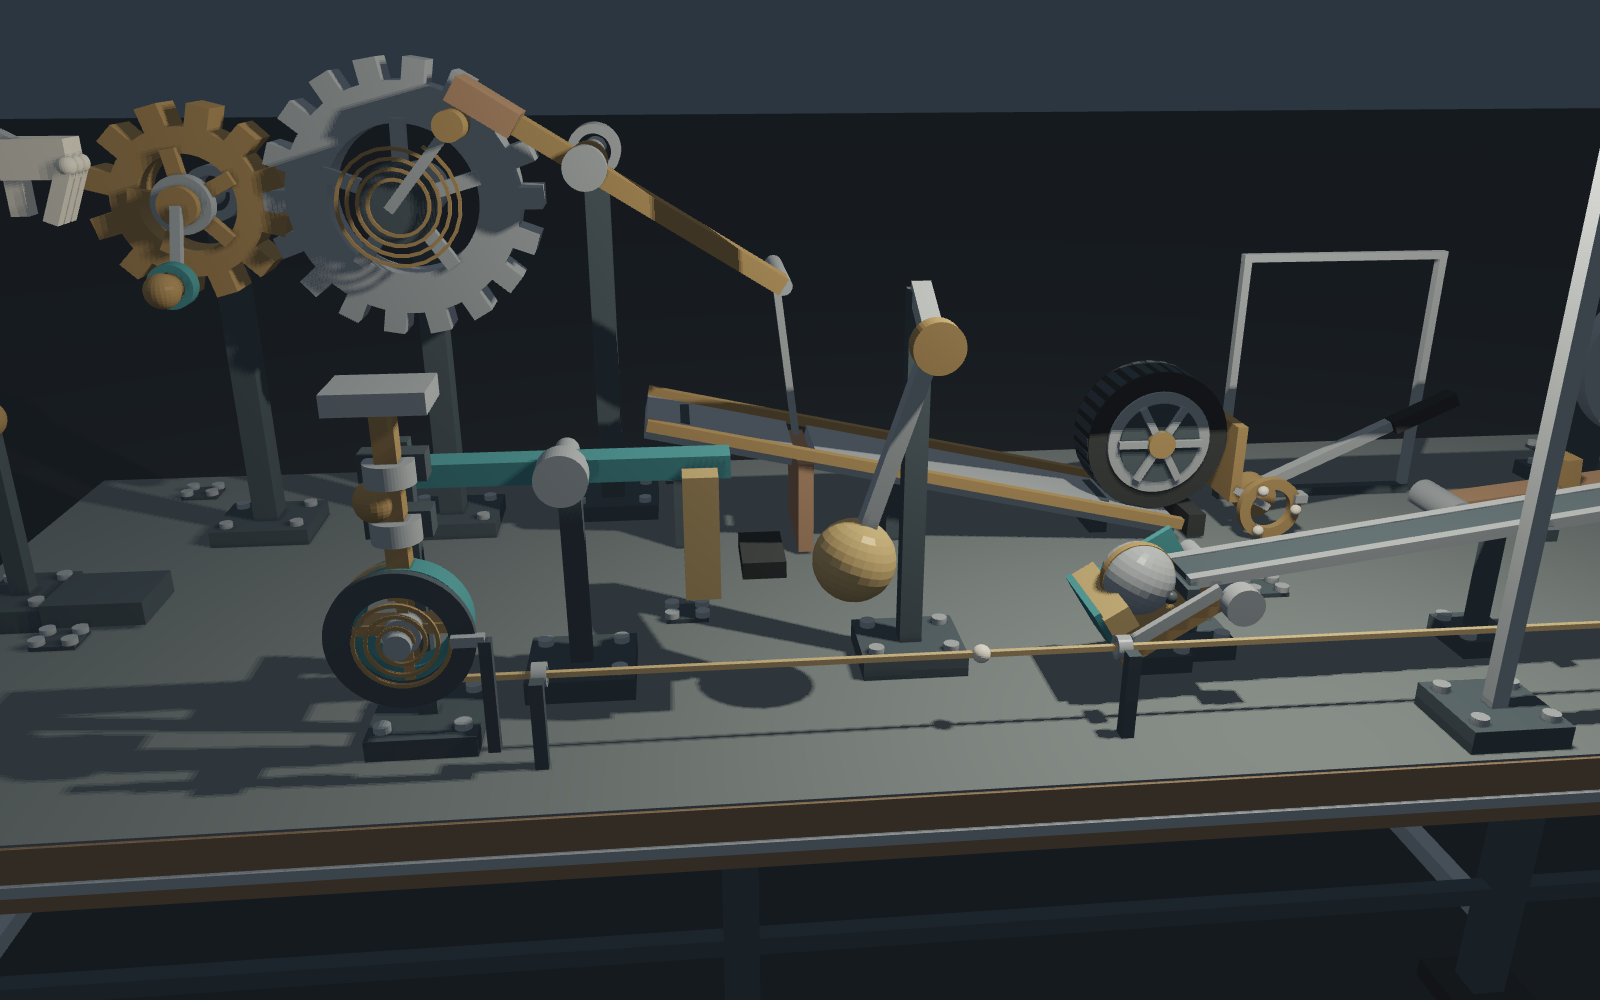
\includegraphics[width=\linewidth,trim={760bp 270bp 325bp 400bp},clip]{figures/shading_1.png}
\captionof{figure}{Flat / face normal: facets on the brass striker and silver relay ball.}
\end{minipage}\hfill\begin{minipage}[t]{.32\linewidth}\vspace{0pt}
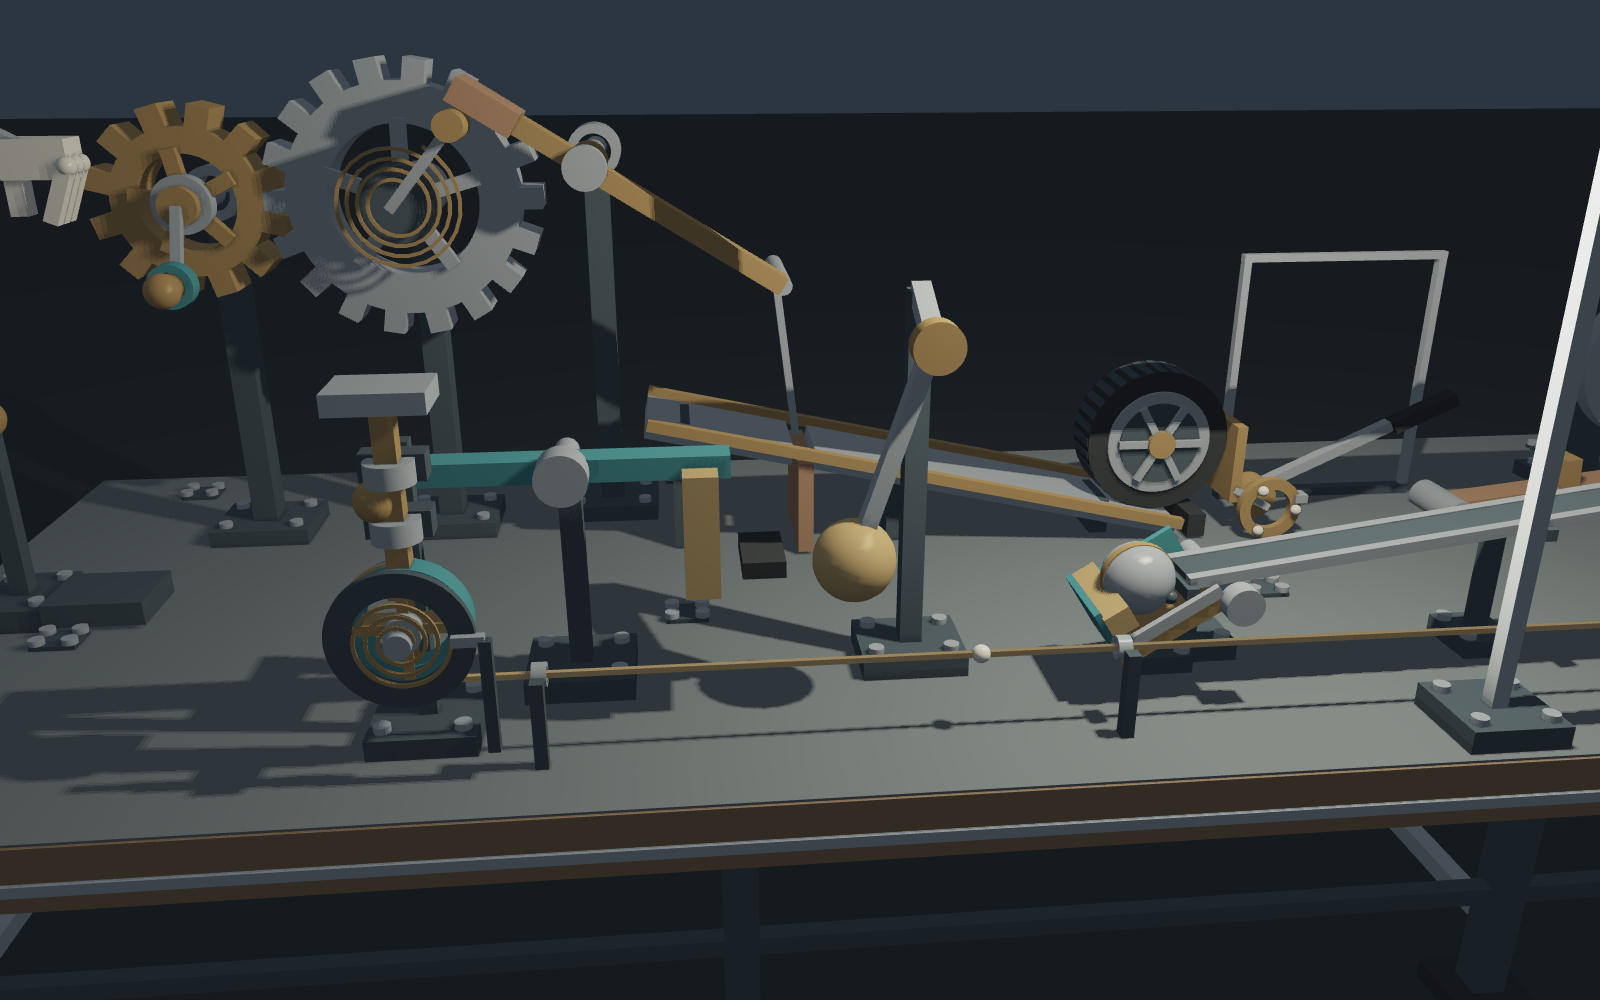
\includegraphics[width=\linewidth,trim={760bp 270bp 325bp 400bp},clip]{figures/shading_2.png}
\captionof{figure}{Gouraud: vertex colors interpolate across each triangle.}
\end{minipage}\hfill\begin{minipage}[t]{.32\linewidth}\vspace{0pt}
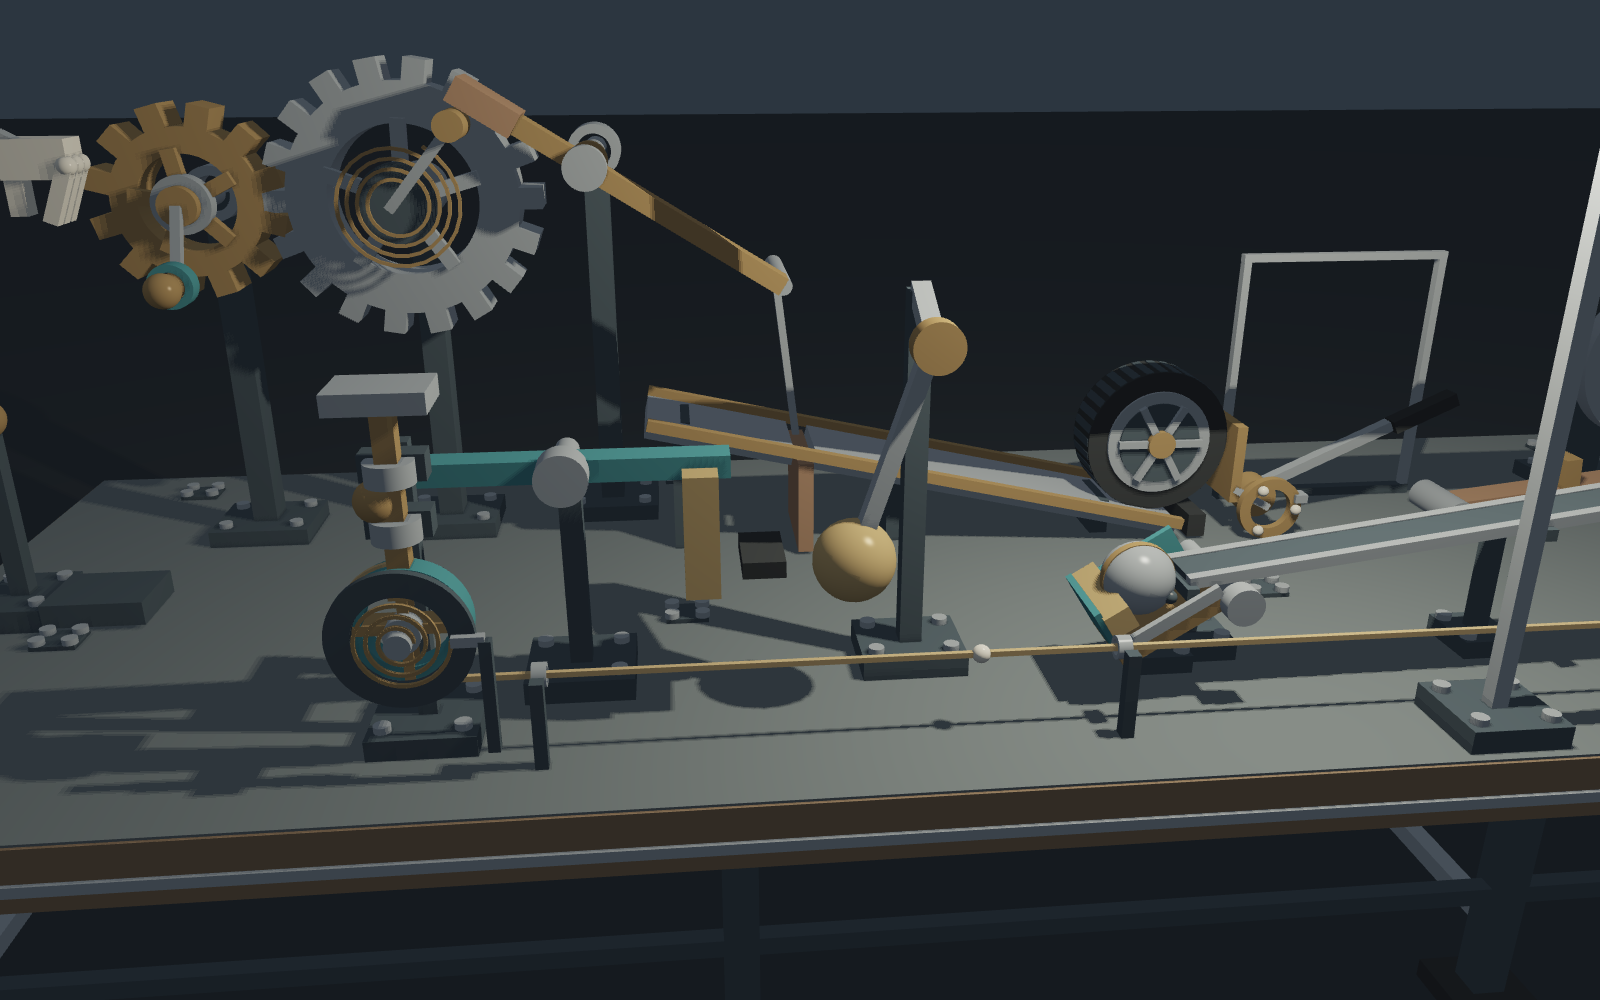
\includegraphics[width=\linewidth,trim={760bp 270bp 325bp 400bp},clip]{figures/shading_0.png}
\captionof{figure}{Phong: interpolated normals provide fragment-level highlights.}
\end{minipage}\par
These matched crops use $t=41$ s, camera 6 and Studio light; only the shading mode changes.
\par\noindent\begin{tabularx}{\linewidth}{@{}p{26mm}Y Y@{}}
\toprule
\textbf{Mode} & \textbf{What the code computes} & \textbf{Expected difference}\\\midrule
Flat / face & Derive a geometric face normal from screen derivatives of world position, then evaluate local lighting per fragment. & Curved meshes look faceted. Point-light distance and shadow visibility may still vary within a triangle.\\
Gouraud & Run \code{evaluateLights()} at each vertex; interpolate separate key, lamp and ambient/emission terms. Apply shadow visibility per fragment. & Smooth color gradients, but the interior of a large triangle cannot discover a highlight missed at its vertices.\\
Phong & Interpolate world position and normal; renormalize the normal, then run the same illumination function in the fragment shader. & Better localization of curved-surface highlights; geometric silhouettes remain polygonal.\\
\bottomrule
\end{tabularx}\par
For perspective-correct weights $\widehat\lambda_i$, the essential distinction is
\begin{align}
\text{Gouraud:}\quad &\mathbf C_j(\mathbf p)=\sum_{i=1}^{3}\widehat\lambda_i\,\mathbf C_{j,i},\\
\text{Phong:}\quad &\mathbf N(\mathbf p)=\operatorname{normalize}\!\left(\sum_{i=1}^{3}\widehat\lambda_i\mathbf N_i\right),
\quad \mathbf C_j=\operatorname{lightTerm}(\mathbf N,\mathbf V,\mathbf L_j,\mathbf E_j).
\end{align}
The displayed Flat mode is a \emph{face-normal lighting mode}, rather than the textbook constant-intensity polygon approximation. This distinction follows the current shader, where $P$, $L$ and $V$ still vary across a face. The L key directly compares Gouraud and Phong; the Light guide button cycles all three modes.
\begin{keyidea}
Keep the camera, pose, material and lamp fixed when comparing shading. Large bench faces are subdivided so Gouraud has enough samples to represent nearby point-light falloff. This improves sampling while preserving vertex-based illumination.
\end{keyidea}

% ------------------------------- 24 / RAY TRACING
\reportpage{CPU ray tracing: a second rendering path}{Press T to trace the current scene and camera into a frozen still with real triangle intersections.}
\twoshots{ray_raster}{OpenGL raster image at $t=70$ s, camera 2, Studio light.}{ray_snapshot}{Matched CPU snapshot: shadow rays and one reflection bounce; internal resolution $800\times500$.}{52mm}
\pic{ray_paths}{49mm}{Ray roles: primary rays choose the visible surface, shadow rays test source visibility, and a reflected ray samples one further scene intersection. No refraction branch is implemented.}
\subsection*{Intersection and acceleration}
Each primary ray is $\mathbf r(\tau)=\mathbf o+\tau\mathbf d$. The M\"oller--Trumbore test solves
\begin{equation}
\mathbf o+\tau\mathbf d=\mathbf a+u(\mathbf b-\mathbf a)+v(\mathbf c-\mathbf a),
\quad u\ge0,\ v\ge0,\ u+v\le1.
\end{equation}
Among valid hits inside the ray's near/far limits, the smallest $\tau$ wins. A binary bounding-volume hierarchy partitions triangle centroids at the median of their widest axis; each leaf contains at most six triangles. Ray/box slab tests reject whole groups before testing their triangles [7,8].
\subsection*{Shading the nearest hit}
Normals are interpolated using the hit's barycentric coordinates and normalized. Direct illumination uses the same material/light equation as the raster path. Shadow rays stop at the lamp distance for point-light visibility. A small normal offset reduces immediate self-intersection.
\[
\mathbf d_r=\mathbf d-2(\mathbf d\cdot\mathbf N)\mathbf N,\qquad
\rho=0.08k_s+0.32m.
\]
At the first hit, when $\rho>0.015$, the non-emissive direct/ambient result is blended with one reflected sample. Secondary hits compute lighting and shadow rays but do not spawn another reflection. Emission is then added. Exposure, tone mapping and gamma produce the stored RGB texture.
\begin{notebox}
\textbf{Snapshot scope:} CPU still image, one primary ray per pixel, at most one reflection bounce. It does not implement path tracing, refraction, diffuse interreflection or ray supersampling. Its exact shadow rays and reflection term can differ from the raster image.
\end{notebox}

% ------------------------------- 25 / INTERACTION
\reportpage{Interactive operation and the demo guide}{The user operates the ready mechanism and can inspect any paused pose from the free camera.}
\pic{guide_operate}{77mm}{The Operate page names the current mechanism and the available input. The top-right Close button is visible, and the bottom status repeats the current action and next instruction.}
\par\noindent\begin{tabularx}{\linewidth}{@{}p{15mm}p{34mm}Y@{}}
\toprule
\textbf{Key} & \textbf{Individual mechanism} & \textbf{Interactive behavior}\\\midrule
G & Glove / starter pin & Hold to grip, carry and place the pin. Releasing the key freezes the partial pose.\\
Z & Gear train & Each press budgets one quarter of the winding stage; four presses complete the turn. Holding does not generate automatic taps.\\
X & Cam / stop lever & Hold to rotate the cam and retract the wheel stop. Release to inspect a partial position.\\
V & Wiper & Hold to sweep the blade toward the clutch bar; release to stop midway.\\
P & Crank & Hold to advance the single compression stroke and raise the ball stop.\\
F & Passive mechanisms & Release the ready wheel, bar or later relay action. It completes and waits at the next stage. F cannot bypass a required held/tapped operation.\\
\bottomrule
\end{tabularx}\par
\subsection*{Six guide pages}
\textbf{Camera} lists navigation and presets; \textbf{Operate} explains the current mechanism; \textbf{Drive} explains the released car; \textbf{Light} controls shadows, shading, exposure and snapshot; \textbf{Chain 1/2} list the full action order, intervals and keys. C, Esc or the Close button dismisses the guide. Opening it alone does not pause the simulation; Space controls pause.
\subsection*{The visible lamp is an interactive object}
The click handler forms a camera ray and finds the nearest scene-triangle hit. Only hits belonging to the lamp's bulb/guard assembly cycle the preset. Foreground geometry prevents clicking through another part. Guide panels, mouse-look mode and snapshots block scene-lamp clicks; B provides a keyboard alternative.
\begin{keyidea}
A button labeled G GUIDE, Z GUIDE, X GUIDE, V GUIDE or P GUIDE opens the instruction page. It does not pretend to perform a held/tapped action. A ready F GO button directly releases its passive mechanism.
\end{keyidea}

% ------------------------------- 26 / DRIVING AND CONTROLS
\reportpage{Keyboard car driving and the controls chart}{The car unlocks after the chain completes. Steering, acceleration and wheel rotation then respond to keyboard input.}
\par\noindent\begin{minipage}[t]{.32\linewidth}\vspace{0pt}
\pic{drive_area}{64mm}{Permitted driving footprint. All four chassis corners must remain on the bay/bridge or apron. The arrow is a schematic driving path.}
\end{minipage}\hfill
\begin{minipage}[t]{.64\linewidth}\vspace{0pt}
\subsection*{Kinematic steering}
With signed travel increment $\Delta s=vh$, front-wheel steer $\delta$ and wheelbase $\ell=2.1$,
\[
\psi'=\psi+\frac{\Delta s\tan\delta}{\ell},\qquad
\mathbf p'=\mathbf p+\Delta s(\cos\psi',0,-\sin\psi').
\]
Throttle changes speed at 3 units/s$^2$, limited to $[-2,3.5]$ units/s; releasing it slows the car at 2.5 units/s$^2$. Steering approaches $\pm0.48$ rad. Steps of at most 0.016 s stabilize edge checks. Rejected moves set speed to zero. Wheel spin is $-d/0.43$.
\end{minipage}\par
\vspace{2mm}
{\small
\par\noindent\begin{tabularx}{\linewidth}{@{}p{38mm}Y p{26mm}@{}}
\toprule
\textbf{Control} & \textbf{Effect} & \textbf{Applies in}\\\midrule
W / S; A / D; Q / E & Camera forward/back; strafe left/right; down/up. & Both modes\\
Hold right mouse & Look; release to restore the UI pointer. Close guide first. & Both; live view\\
Left Shift; scroll & Faster camera; scroll moves along view direction with guide closed. & Both; live view\\
1 / 2 / 3 & Overview / crank / glove and gears. & Both modes\\
4 / 5 / 6 & Car/apron / front row / relay contacts. & Both modes\\
I; Mode button & Switch presentation/interactive and reset. & Both modes\\
Space; Play/Pause & Pause/resume; release ready F action; show required-key guide when appropriate. & Both modes\\
R; Reset button & Reset mechanisms, car, queued turns and held keys. & Both modes\\
G / Z / X / V / P & Individual hold/tap operations (page 25). & Interactive only\\
F; F GO button & Release the current passive action. & Interactive only\\
Up / Down & Accelerate / brake, then reverse. & Both, after release\\
Left / Right & Steer front wheels; arrow input takes over automatic exit. & Both, after release\\
C; Guide; Close & Open/close six-page guide. & Both modes\\
Esc & Close guide and release captured mouse. & Live view\\
H & Toggle numbered object labels. & Both modes\\
Lamp click; B & Studio $\rightarrow$ Daylight $\rightarrow$ Sunset $\rightarrow$ Night. & Both; live view\\
L & Compare Phong and Gouraud. & Both; live view\\
Light-page buttons & Shadows on/off, three shading modes, exposure $-/+$, snapshot. & Both; guide open\\
T & Trace the current pose and camera. & Both; live view\\
T / Esc / left click & Return from snapshot and restore prior run state. & Snapshot only\\
Window X / Alt+F4 & Close the application through the window system. & Application\\
\bottomrule
\end{tabularx}\par}
\textbf{Driving conditions:} the simulation must be running and the car released. Drive straight over the bridge before turning. WASD/QE continue controlling the camera independently; snapshots freeze camera and driving interaction.

% ------------------------------- 27 / ARCHITECTURE
\reportpage{Program architecture and the rendering pipeline}{Both rendering paths consume the same posed scene, which keeps geometry, materials and camera settings consistent.}
\pic{architecture}{54mm}{Application data flow. CPU simulation supplies transformed draw items; OpenGL rasterization and the optional CPU tracer use those items to produce the displayed image.}
\par\noindent\begin{tabularx}{\linewidth}{@{}p{29mm}Y Y@{}}
\toprule
\textbf{Source file} & \textbf{Responsibility} & \textbf{Key data / behavior}\\\midrule
\code{math3d.h} & Vector and matrix mathematics. & Column-major matrices, TRS, lookAt, perspective, ray direction.\\
\code{animation.h} & Poses, mechanism controller, camera and car. & Stage times, interpolation, contact guards, held/tapped controls.\\
\code{scene.h} & Build visible assemblies. & Mesh index + model matrix + material per draw item.\\
\code{lighting.h} & Shared environment parameters. & Lamp position, source energies, ambient, exposure, background.\\
\code{renderer.h} & Mesh upload, shaders, shadows and picking. & Eight reusable meshes, depth passes, three shading branches.\\
\code{raytrace.h} & CPU snapshot. & World triangles, BVH, hit/shadow/reflection rays, image texture.\\
\code{hud.h} & Guide and status overlay. & Built-in bitmap glyphs drawn as tiny triangle rectangles; shared layout/hit bounds.\\
\code{main.cpp} & Window, callbacks and frame loop. & GLFW context/time, independent camera input, scene rebuild, rendering, captures.\\
\code{validation.h} & Verification routines. & Numerical tests, adverse handoffs, GPU shadow tests and handler checks.\\
\bottomrule
\end{tabularx}\par
\subsection*{Live rendering, in order}
\begin{enumerate}
\item Poll input and update permitted simulation time, camera and car state.
\item Evaluate the mechanism pose and assemble the draw list from reusable meshes.
\item Render source depth maps, then transform scene vertices with $PVM$.
\item Rasterize triangles, interpolate shader outputs, evaluate shading/visibility and depth-test fragments.
\item Apply tone/gamma conversion; draw the guide/status overlay and swap buffers.
\end{enumerate}
The depth buffer resolves visible opaque surfaces. The program requests four-sample MSAA for geometric edges; this is a context request, not a measured guarantee of a particular sample count on every machine. Scene geometry is opaque; a texture is used to display the already-computed ray image.
\textbf{Build environment:} C++17, MinGW g++, GLFW 3, GLAD and OpenGL 3.3 Core / GLSL 330. \code{mingw32-make build} builds \code{cog_demo.exe}; \code{run.bat} rebuilds and launches. The prepared submission directory also contains the runtime DLLs.

% ------------------------------- 28 / VERIFICATION
\reportpage{Verification and measured evidence}{Geometric checks, actual GPU tests and visual inspection answer different questions; all three are useful.}
\par\noindent\begin{tabularx}{\linewidth}{@{}p{35mm}Y p{28mm}@{}}
\toprule
\textbf{Check} & \textbf{What was verified} & \textbf{Observed result}\\\midrule
Geometry, controller, UI & Correct and obstructed handoffs; transformation order, input rules, reset, car and guide behavior. & 472 focused assertions passed.\\
Pose continuity sweep & 9,241 poses sampled at 120 samples/s over the 77-second sequence; rod/cable lengths, rolling, continuity and exit conditions. & 189,430 repeated numeric invariants passed.\\
Projection consistency & Six presets, three aspect ratios, nine image locations; ray-to-screen round trips and near/far endpoints. & Passed within test tolerances.\\
Normals and mesh orientation & Inverse-transpose perpendicularity; all eight reusable meshes' triangle winding and nondegeneracy. & 54,188 mesh triangles checked.\\
Lamp cubemap & Each of six directions measures a box face 1.5 units from the lamp. & Radial depth error below 0.002 units.\\
GPU visibility & Add a blocker, compare lit/shadowed receiver in all three shading modes, then remove blocker. & Occlusion and restored lighting passed.\\
Full interactive run & Real handlers, required held/tapped inputs, complete ordered chain and car departure. & Release at 70.0000 active s; exit passed; 420 GPU frames.\\
Snapshot capture & Current scene at $t=70$ s, camera 2, Studio, $800\times500$ CPU image. & 165,980 world triangles; 1,893.63 ms in one local capture.\\
\bottomrule
\end{tabularx}\par
\subsection*{Reproducible commands}
\begin{lstlisting}
mingw32-make test
.\cog_demo.exe --verify-lighting
.\cog_demo.exe --verify-interactive
.\cog_demo.exe --verify-timing
\end{lstlisting}
The first three commands were rerun during the project assessment. The dedicated report capture harness reused the unchanged scene and renderer for matched screenshots and the snapshot measurement. Its output manifest records pose, camera, lighting and shading for each capture. Source-file hashes are included in the report package.
\subsection*{How to interpret the numbers}
The interactive verification advances simulated time in fixed 0.2-second increments, so its short wall time is \emph{not} a real-time playback measurement. Its 420 frames demonstrate complete rendered state progression and handler execution. Use \code{--verify-timing} to check wall-clock playback on the target machine.

The local GPU identifies as Intel Iris Xe, OpenGL 3.3.0, driver build 31.0.101.4502. Snapshot time is one observation, including scene preparation and tracing; it is not a repeated benchmark or a promise for other hardware. The 54,188 mesh-library triangles differ from the larger instanced world-triangle count.
\begin{keyidea}
Numeric tests establish mathematical and state consistency. Matched screenshots separately establish framing, readable contacts and visible lighting/shading differences. A large assertion count alone is not evidence of visual quality.
\end{keyidea}

% ------------------------------- 29 / DEMONSTRATION
\reportpage{Demonstration plan, results and limitations}{A short, deliberate demonstration should expose both the causal machine and the graphics behind its image.}
\twoshots{complete}{Completed mechanism immediately before car departure.}{car_exit}{Visible outcome: the car has crossed the lowered bridge.}{49mm}
\par\noindent\begin{tabularx}{\linewidth}{@{}p{10mm}p{33mm}Y@{}}
\toprule
 & \textbf{Show} & \textbf{Explain / demonstrate}\\\midrule
1 & Overview, preset 1 & Identify the back row, returning front relay, cable and car bay. Start the 70-second sequence.\\
2 & Pause + preset 3 & Glove attachment, cube gear teeth and local pivot transforms. Use L for a fixed-view Gouraud/Phong comparison.\\
3 & Presets 2 and 6 & Crank rod length, ball-to-cup transfer, early striker release, rocker collar contact and drum take-up.\\
4 & Click lamp / B & Same scene under four environments; explain the visible point source, added sun and independent shadows.\\
5 & Preset 4 and arrows & Barrier clearance, bridge endpoint, withdrawn coupling and shoe; then steer the released car onto the apron.\\
6 & I, G, Z, X, V, P & Reset to interactive mode; stop a held operation halfway and resume it. Show that a future key cannot skip the current stage.\\
7 & C and T & Show the guide's current action and next instruction. Trace a still, then return with the prior play/pause state preserved.\\
\bottomrule
\end{tabularx}\par
\subsection*{What the completed project demonstrates}
The chain combines distinct rotational, sliding, rolling and hinged motions with visible contacts. A common hierarchy connects part construction to animation; a shared lighting equation connects material parameters to both raster and ray images. Camera movement, mechanism operation, lighting comparison and car driving provide different forms of interaction.
\subsection*{Boundaries of the implementation}
\begin{itemize}
\item \textbf{Mechanics:} deterministic authored kinematics and selected handoff tests. Spring force, hydraulic pressure, general rigid-body collisions and engine dynamics are not solved.
\item \textbf{Lighting:} point-source lamp, approximate ambient, finite shadow maps and heuristic metallic response. Physical area lights and diffuse global illumination are outside scope.
\item \textbf{Shading/modeling:} smooth shading does not remove polygonal silhouettes. The Flat button selects face-normal lighting. The cabin remains opaque, without refraction or surface image textures.
\item \textbf{Driving/snapshot:} all wheels share chassis travel; no differential or tire dynamics. Ray tracing is an $800$-pixel-wide still with one reflection bounce.
\end{itemize}
Possible extensions include a selectable orthographic inspection view, more direct interactions for the passive relay, adaptive mesh detail, and higher-quality snapshot sampling. These are future work rather than present features.

% ------------------------------- 30 / CONCLUSION + REFERENCES
\reportpage{Conclusion and references}{The project turns the course pipeline into an observable machine: geometry becomes motion, motion is projected, and illumination becomes color.}
The completed application demonstrates procedural object construction, homogeneous 3D transformations, parent/child motion, perspective viewing, local illumination, shading comparisons, shadow visibility and triangle ray tracing in one coherent scene. Its seventeen-action chain reaches the release condition at 70 active seconds and produces a car that the user can drive. Interactive controls preserve the same order and reset rules as the presentation.

The report connects each major claim to a visible object, an implemented equation, a control or a measured check. This connection is the central result: the reader can follow the chain first, then trace its appearance and behavior back to the graphics calculations.
\subsection*{References and implementation sources}
{\small
\begin{enumerate}[label={[\arabic*]},leftmargin=21pt,itemsep=6pt]
\item \textbf{Supplied course lectures.} \emph{L3 3D Transformation v2}; \emph{L4 3D Viewing2}; \emph{L5 Projection v2}; \emph{L6 Projective transform}; \emph{L8 Illumination}; \emph{L9 shading}. Course material supplied for this report. Used for the transformation, viewing, projection, illumination and shading framework.
\item \textbf{Project implementation.} \StudentName, \emph{Interactive Automotive Chain Reaction}, C++17/OpenGL source snapshot. Principal files: \code{animation.h}, \code{scene.h}, \code{math3d.h}, \code{renderer.h}, \code{lighting.h}, \code{raytrace.h}, \code{hud.h}, \code{main.cpp}, \code{validation.h}. Included report manifests identify source hashes and screenshot parameters.
\item \textbf{The Khronos Group.} \emph{The OpenGL Graphics System: A Specification, Version 3.3 Core Profile}, 11 March 2010. Background for vertex processing, interpolation, clipping, depth and rasterization.\\
\url{https://registry.khronos.org/OpenGL/specs/gl/glspec33.core.pdf}
\item \textbf{GLFW.} \emph{GLFW 3.3 Input Guide}. Background for callbacks, key states, mouse input and cursor modes.\\
\url{https://www.glfw.org/docs/3.3/input_guide.html}
\item \textbf{Bui Tuong Phong.} ``Illumination for Computer Generated Pictures,'' \emph{Communications of the ACM}, 18(6), pp. 311--317, 1975.\\
\url{https://doi.org/10.1145/360825.360839}
\item \textbf{Henri Gouraud.} ``Continuous Shading of Curved Surfaces,'' \emph{IEEE Transactions on Computers}, C-20(6), pp. 623--629, 1971.\\
\url{https://doi.org/10.1109/T-C.1971.223313}
\item \textbf{Tomas M\"oller and Ben Trumbore.} ``Fast, Minimum Storage Ray-Triangle Intersection,'' \emph{Journal of Graphics Tools}, 2(1), pp. 21--28, 1997.\\
\url{https://doi.org/10.1080/10867651.1997.10487468}
\item \textbf{Matt Pharr, Wenzel Jakob and Greg Humphreys.} \emph{Physically Based Rendering: From Theory to Implementation}, 4th ed., 2023. ``pbrt: System Overview.'' Used for general ray/visibility and acceleration-structure context; this project implements the smaller snapshot scope stated on page 24.\\
\url{https://pbr-book.org/4ed/Introduction/pbrt_System_Overview}
\end{enumerate}}
\label{report:lastpage}
\end{document}
